%encoding UTF-8
\author{Евгений Синельников, Игорь Чудов}
\city{Саратов}
\affiliation{Базальт СПО}
\projecttitle{ALT Join}
\projecturl{\url{http://altlinux.org/}}
\title{Приобщение к участию в разработке свбодных программ на примере
стажировки в компании Базальт СПО}
\maketitle

\begin{abstract}
  В рамках доклада рассмотрена проблема обучения новых
  сотрудников в компаниях, работающих с СПО. Предложены методики для
  ускорения процедуры включения людей в рабочие процессы. Представлены
  примеры вводных документов.
\end{abstract}


\section{Проблематика}

В сравнении с компаниями, ориентированными на outsource-разработку для
множества различных заказчиков, небольшие продуктовые компании
испытывают дефицит кадров.

Исходные данные для анализа представляют из себя выборку заявок на Join
с сайта http://bugzilla.altlinux.org/ за весь доступный период (2008-2020 годы):

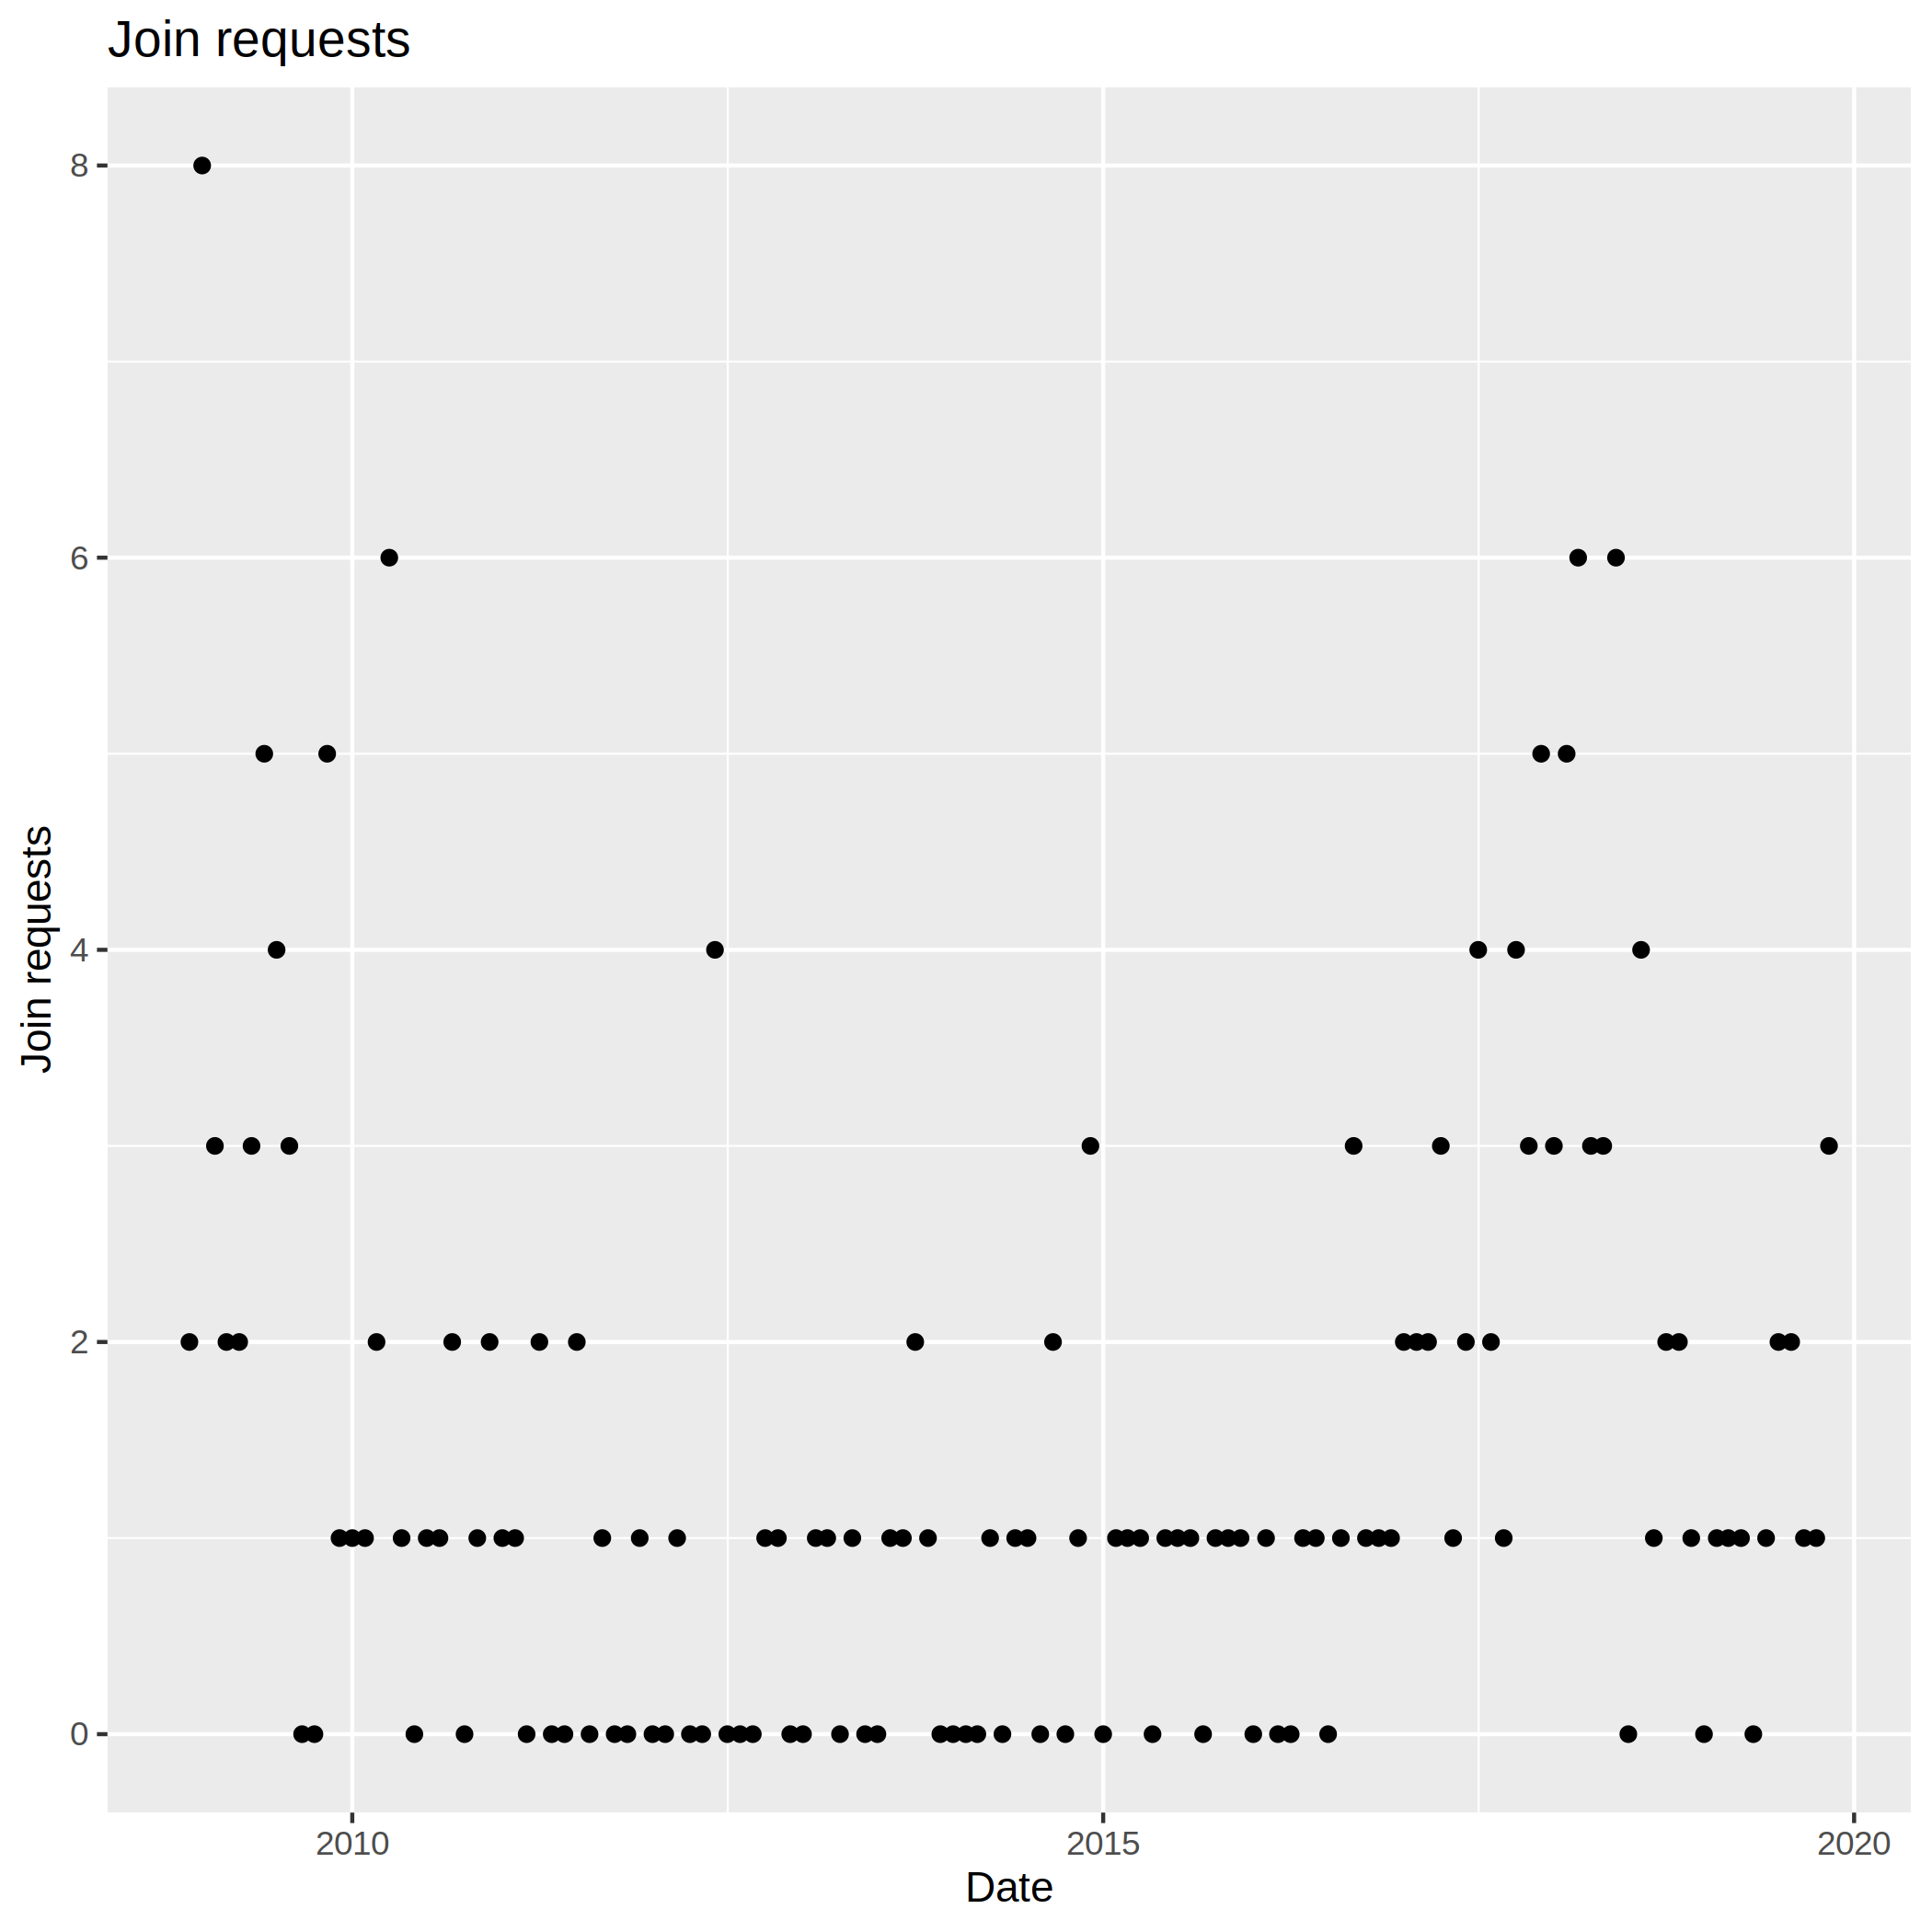
\includegraphics{ggplot}

Не смотря на длительный период выборки можно отметить, что количество
поступающих заявок невелико, что может служить сигналом о нескольких
проблемах:

\begin{itemize}
\item Проблема с процедурой подачи заявок (неочевидность, сложность,
бюрократия, длительность).
\item Проблема с методом коммуникации (устаревание инструмента и
методики).
\item Также сказывается специфика предметной области с которой связана
работа.
\end{itemize}

Поступающие кадры недообучены и незнакомы с базовыми понятиями отрасли,
также не воспринимают принятые в сообществе разработчиков СПО средства
коммуникации.


\section{Методы решения проблемы}

Для ускорения процедуры адаптации сотрудников были опробованы следующие
методы:

- Раздаточные материалы: одностраничная брошюра с базовыми ссылками и
  программами, на которой сотрудник может сделать пометки.
- Коллективно дополняемые HOWTO.
- Менторинг.


\begin{enumerate}
\item Создание файлов конфигурации для сборки ( \Q{make-config.sh} );
\item Сборка кросс-компилятора Common LISP. Данная часть называется
GENESIS 1;
\item Сборка компонентов целевого компилятора: эта часть собирается после
GENESIS 1, чтобы получить файл \Q{sbcl.h} для сборки части, написанной на
С, и до сборки GENESIS 2, чтобы получить таблицу символов.
\item Запускается кросс-компилятор для получения объектных файлов для
целевой операционной платформы.
\item Запускается GENESIS 2, чтобы получить \Q{cold-sbcl.core}.
Создаётся с помощью \Q{src/compiler/generic/genesis.lisp}, который
преобразует FASL файлы в образ LISP-системы на хосте.
\item Производится warm init - загрузка и сборка CLOS
( \EN{Common LISP Object System} ), а также компонентов, от неё зависящих.
\end{enumerate}

Для успешного прохождения всех этапов необходимо реализовать часть
системы, которая зависит от целевой архитектуры.


\section{Части системы}

SBCL технически является компилятором - каждое поступающее на вход
выражение сначала проходит этап компиляции в двоичный код, и только потом
исполняется. Соответственно, для выполнения этой задачи в SBCL
существует платформо-зависимая часть.

Платформо-зависимая часть состоит из определения регистров в файле
\Q{src/runtime/platformname-lispregs.h} , где \Q{platformname} -
название целевой архитектуры. Этот элемент необходим для описания
доступных для работы регистров.

Также существует ассемблерная часть в файле
\Q{src/runtime/platformname-assem.S}, где определены всего две функции -
\Q{call_into_c} и \Q{call_into_lisp}, которые выполняют переключение
между C и SBCL ABI. Одна из задач этой части - переключение на
C runtime, который отвечает за обработку сигналов, полученныx от
операционной системы. Для реализации таковых функций необходимо хорошее
знание \EN{platform ABI} целевой архитектуры, а также особенностей
целевой операционной системы.

Самая объёмная и сложная платформо-зависимая часть системы находится в
директориях \Q{src/assembly/platformname} и \Q{src/compiler/platformname}
и содержит определения виртуальных операций (VOP) которые необходимы,
чтобы преобразовать код на LISP в ассемблерный код, и используются в
виртуальной машине SBCL в качестве низкоуровневых операций для
в стандартных функциях ANSI Common LISP.

Одним из плюсов использования \EN{Virtual OPerations} является
возможность получать детализированные ассемблерные листинги при вызове
дизассемблирования.


\section{Проблемы при портировании на архитектуру e2k}

В ситуации с портированием SBCL на архитектуру e2k в ОС ALT Linux были
обнаружены следующие проблемы:

\begin{itemize}
\item Отсутствие кросс-компилятора C. Многие компиляторы, как SBCL, GHC
и другие, не рассчитаны на сборку только на целевой платформе;
\item Отсутствие детальной документации на C ABI для e2k. Данное знание
необходимо для реализации функции переключения между SBCL ABI и C ABI,
а также для эффективной реализации VOPs. Некоторые вещи приходится
изучать методом исследования ассемблерных листингов;
\item Частично утеряна документация по SBCL internals. К сожалению,
лучшее средство изучения проекта - чтение кода и общение в списках
рассылки;
\item Сложность ручного просчёта блоков инструкций для широких слов.
Ассемблер e2k плохо подходит для написания кода вручную;
\end{itemize}


\section{Библиография}

\begin{thebibliography}{9}
\bibitem{cliki} SBCL Internals CLiki site.
\url{https://web.archive.org/web/20120814000933/http://sbcl-internals.cliki.net/index}
\end{thebibliography}


%%% Local Variables: 
%%% mode: latex
%%% TeX-master: "../main"
%%% End: 
